\lab{Pandas 1: Introduction}{Pandas 1: Introduction}
\labdependencies{}
\objective{Though NumPy and SciPy are powerful tools for numerical computing, they lack some of the high-level functionality necessary for many data science applications.
Python's \emph{pandas} library, built on NumPy, is designed specifically for data management and analysis.
In this lab we introduce pandas data structures and syntax, and we explore the capabilities of pandas for quickly analyzing and presenting data.
}
\label{lab:pandas1}

\section*{Pandas Basics}

Pandas is a python library used primarily to analyze data.
It combines functionality of NumPy, MatPlotLib, and SQL to create an easy to understand library that allows for the manipulation of data in various ways.
In this lab we focus on the use of Pandas to analyze and manipulate data in ways similar to NumPy and SQL.

\subsection*{Pandas Data Structures}

\subsubsection*{Series}

The first pandas data structure is a \li{Series}.
A \li{Series} is a one-dimensional array that can hold any datatype, similar to an \li{ndarray}.
However, a \li{Series} has an explicitly defined \li{index} that gives a label to each entry.
An \li{index} generally is used to label the data.

Typically a \li{Series} contains information about one feature of the data.
For example, the data in a \li{Series} might show a class's grades on a test and the \li{Index} would indicate each student in the class.
To initialize a \li{Series}, the first parameter is the data and the second is the index.

\begin{lstlisting}
>>> import pandas as pd
>>> import numpy as np
# Initialize Series of student grades
>>> math = pd.Series(np.random.randint(0, 100, 4), ["Mark", "Barbara",
...		"Eleanor", "David"])
>>> english = pd.Series(np.random.randint(0, 100, 5), ["Mark", "Barbara",
...		"David", "Greg", "Lauren"])
\end{lstlisting}

\subsubsection*{DataFrame}

The second key pandas data structure is a \li{DataFrame}.
A \li{DataFrame} is a collection of multiple \li{Series}.
It can be thought of as a 2-dimensional array, where each row is a separate datapoint and each column is a feature of the data.
The rows are labeled with an \li{index} (as in a \li{Series}) and the columns are labeled in the attribute \li{columns}.

There are many different ways to initialize a \li{DataFrame}.
One way to initialize a \li{DataFrame} is by passing in a dictionary as the data of the \li{DataFrame}.
The keys of the dictionary will become the labels in \li{columns} and the values are the \li{Series} associated with the label.

\begin{lstlisting}
# Create a DataFrame of student grades
>>> grades = pd.DataFrame({"Math": math, "English": english})
>>> grades
	      Math  English
Barbara   52.0     73.0
David     10.0     39.0
Eleanor   35.0      NaN
Greg       NaN     26.0
Lauren     NaN     99.0
Mark      81.0     68.0
\end{lstlisting}

Notice that \li{pd.DataFrame} automatically lines up data from both \li{Series} that have the same index.
If the data only appears in one of the \li{Series}, the corresponding entry for the other \li{Series} is \li{NaN}.

We can also initialize a \li{DataFrame} with a NumPy array.
With this method, the data is passed in as a 2-dimensional NumPy array, while the column labels and the index are passed in as parameters.
The first column label goes with the first column of the array, the second with the second, and so forth.
The index works similarly.

\begin{lstlisting}
# Initialize DataFrame with NumPy array. This is identical to the grades DataFrame above.
>>> data = np.array([[52.0, 73.0], [10.0, 39.0], [35.0, np.nan],
...		[np.nan, 26.0], [np.nan, 99.0], [81.0, 68.0]])
>>> grades = pd.DataFrame(data, columns = ["Math", "English"], index =
...		["Barbara", "David", "Eleanor", "Greg", "Lauren", "Mark"])

# View the columns
>>> grades.columns
Index(["Math", "English"], dtype="object")

# View the Index
>>> grades.index
Index(["Barbara", "David", "Eleanor", "Greg", "Lauren", "Mark"], dtype="object")
\end{lstlisting}

\pagebreak

A \li{DataFrame} can also be viewed as a NumPy array using the attribute \li{values}.

\begin{lstlisting}
# View the DataFrame as a NumPy array
>>> grades.values
array([[ 52.,  73.],
       [ 10.,  39.],
       [ 35.,  nan],
       [ nan,  26.],
       [ nan,  99.],
       [ 81.,  68.]])
\end{lstlisting}

\subsection*{Data I/O}

The pandas library has functions that make importing and exporting data simple.
The functions allow for a variety of file formats to be imported and exported, including CSV, Excel, HDF5, SQL, JSON, HTML, and pickle files.

\begin{table}[H]
\begin{tabular}{r|l}
Method & Description \\ \hline
\li{to_csv()}    & Write the index and entries to a CSV file \\
\li{read_csv()}  & Read a csv and convert into a DataFrame\\
\li{to_json()}   & Convert the object to a JSON string \\
\li{to_pickle()} & Serialize the object and store it in an external file \\
\li{to_sql()}    & Write the object data to an open SQL database \\
\li{read_html()} & Read a table in an html page and convert to a DataFrame\\
\end{tabular}
\caption{Methods for exporting data in a pandas \li{Series} or \li{DataFrame}.}
\label{table:pandas-view-or-export}
\end{table}

The CSV (comma separated values) format is a simple way of storing tabular data
in plain text.
Because CSV files are one of the most popular file formats for exchanging data, we will explore the \li{read_csv()} function in more detail.
Some frequently-used keyword arguments include the following:

\begin{itemize}
\item \li{delimiter}:
The character that separates data fields. It is often a
comma or a whitespace character.
\item \li{header}: The row number (0 indexed) in the CSV file that contains the column names.
 \item \li{index_col}: The column (0 indexed) in the CSV file that is the index for the
\li{DataFrame}.
 \item \li{skiprows}:
If an integer $n$, skip the first $n$ rows of the file, and then start reading
in the data.
If a list of integers, skip the specified rows.
 \item \li{names}:
If the CSV file does not contain the column names, or you wish to use other
column names, specify them in a list.
\end{itemize}

Another particularly useful function is \li{read_html()}, which is useful when scraping data.
It takes in a url or html file and an optional argument \li{match}, a string or regex, and returns a list of the tables that match the \li{match} in a DataFrame.

\section*{Data Manipulation}

\subsection*{Accessing Data}

In general, the best way to access data in a \li{Series} or \li{DataFrame} is through the indexers \li{loc} and \li{iloc}.
While array slicing can be used, it is more efficient to use these indexers.
Accessing \li{Series} and \li{DataFrame} objects using these indexing operations is more efficient than slicing because the bracket indexing has to check many cases before it can determine how to slice the data structure.
Using \li{loc} or \li{iloc} explicitly bypasses these extra checks.
The \li{loc} index selects rows and columns based on their labels, while \li{iloc} selects them based on their integer position.
With these indexers, the first and second arguments refer to the rows and columns, respectively, just as array slicing.

\begin{lstlisting}
# Use loc to select the Math scores of David and Greg
>>> grades.loc[["David", "Greg"], "Math"]
David    10.0
Greg      NaN
Name: Math, dtype: float64

# Use iloc to select the Math scores of David and Greg
>>> grades.iloc[[1,3], 0]
David    10.0
Greg      NaN
\end{lstlisting}

To access an entire column of a \li{DataFrame}, the most efficient method is to use only square brackets and the name of the column, without the indexer.
This syntax can also be used to create a new column or reset the values of an entire column.

\begin{lstlisting}
# Create a new History column with array of random values
>>> grades["History"] = np.random.randint(0, 100, 6)
>>> grades["History"]
Barbara     4
David      92
Eleanor    25
Greg       79
Lauren     82
Mark       27
Name: History, dtype: int64

# Reset the column such that everyone has a 100
>>> grades["History"] = 100.0
>>> grades
         Math  English  History
Barbara  52.0     73.0    100.0
David    10.0     39.0    100.0
Eleanor  35.0      NaN    100.0
Greg      NaN     26.0    100.0
Lauren    NaN     99.0    100.0
Mark     81.0     68.0    100.0
\end{lstlisting}

Datasets can often be very large and thus difficult to visualize.
Pandas has various methods to make this easier.
The methods \li{head} and \li{tail} will show the first or last $n$ data points, respectively, where $n$ defaults to 5.
The method \li{sample} will draw $n$ random entries of the dataset, where $n$ defaults to 1.
\begin{lstlisting}
# Use head to see the first n rows
>>> grades.head(n=2)
         Math  English  History
Barbara  52.0     73.0    100.0
David    10.0     39.0    100.0

# Use sample to sample a random entry
>>> grades.sample()
        Math  English  History
Lauren   NaN     99.0    100.0
\end{lstlisting}
It may also be useful to re-order the columns or rows or sort according to a
given column.
\begin{lstlisting}
# Re-order columns
>>> grades.reindex(columns=["English", "Math", "History"])
         English  Math  History
Barbara     73.0  52.0    100.0
David       39.0  10.0    100.0
Eleanor      NaN  35.0    100.0
Greg        26.0   NaN    100.0
Lauren      99.0   NaN    100.0
Mark        68.0  81.0    100.0

# Sort descending according to Math grades
>>> grades.sort_values("Math", ascending=False)
         Math  English  History
Mark     81.0     68.0    100.0
Barbara  52.0     73.0    100.0
Eleanor  35.0      NaN    100.0
David    10.0     39.0    100.0
Greg      NaN     26.0    100.0
Lauren    NaN     99.0    100.0
\end{lstlisting}
Other methods used for manipulating \li{DataFrame} and \li{Series} panda structures can be found in Table \ref{table:pandas-manage-data}.
\begin{table}[H]
\begin{tabular}{r|l}
Method & Description \\ \hline
\li{append()} & Concatenate two or more \li{Series}. \\
\li{drop()} & Remove the entries with the specified label or labels \\
\li{drop_duplicates()} & Remove duplicate values \\
\li{dropna()} & Drop null entries \\
\li{fillna()} & Replace null entries with a specified value or strategy \\
\li{reindex()} & Replace the index \\
\li{sample()} & Draw a random entry \\
\li{shift()} & Shift the index \\
\li{unique()} & Return unique values \\
\end{tabular}
\caption{Methods for managing or modifying data in a pandas \li{Series} or \li{DataFrame}.}
\label{table:pandas-manage-data}
\end{table}

\begin{problem}
The file \li{budget.csv} contains the budget of a college student over the course of 4 years.
Write a function that performs the following operations in this order:
\begin{enumerate}
\item Read in \li{budget.csv} as a \li{DataFrame} with the index as column 0. Hint: Use \li{index\_col=0} to set the first column as the index when reading in the csv.
\item Reindex the columns such that amount spent on groceries is the first column and all other columns maintain the same ordering.
\item Sort the \li{DataFrame} in descending order by how much money was spent on \li{Groceries}.
\item Reset all values in the \li{"Rent"} column to \li{800.0}.
\item Reset all values in the first 5 data points to \li{0.0}.
\end{enumerate}
Return the values of the updated \li{DataFrame} as a NumPy array.

\label{prob:budget}
\end{problem}

\subsection*{Basic Data Manipulation}
Because the primary pandas data structures are based off of \li{ndarray}, most NumPy functions work with pandas structures.
For example, basic vector operations work as would be expected:

\begin{lstlisting}
# Sum history and english grades of all students
>>> grades["English"] + grades["History"]
Barbara    173.0
David      139.0
Eleanor      NaN
Greg       126.0
Lauren     199.0
Mark       168.0
dtype: float64

# Double all Math grades
>>>  grades["Math"]*2
Barbara    104.0
David       20.0
Eleanor     70.0
Greg         NaN
Lauren       NaN
Mark       162.0
Name: Math, dtype: float64
\end{lstlisting}
In addition to arithmetic, \li{Series} has a variety of other methods similar to NumPy arrays.
A collection of these methods is found in Table \ref{table:pandas-numerical-methods}.
\begin{table}[H]
\begin{tabular}{r|l}
Method & Returns \\ \hline
\li{<<abs>>()}     & Object with absolute values taken (of numerical data) \\
\li{idxmax()}  & The index label of the maximum value \\
\li{idxmin()}  & The index label of the minimum value \\
\li{count()}   & The number of non-null entries \\
\li{cumprod()} & The cumulative product over an axis \\
\li{cumsum()}  & The cumulative sum over an axis \\
\li{<<max>>()}     & The maximum of the entries \\
\li{mean()}    & The average of the entries \\
\li{median()}  & The median of the entries \\
\li{<<min>>()}     & The minimum of the entries \\
\li{mode()}    & The most common element(s) \\
\li{prod()}    & The product of the elements \\
\li{<<sum>>()}     & The sum of the elements \\
\li{var()}     & The variance of the elements \\
\end{tabular}
\caption{Numerical methods of the \li{Series} and \li{DataFrame} pandas classes.}
\label{table:pandas-numerical-methods}
\end{table}

\subsection*{Basic Statistical Functions}

The pandas library allows us to easily calculate basic summary statistics of our data,
which can be useful when we want a quick description of the data.
The \li{describe()} function
outputs several such summary statistics for each column in a \li{DataFrame}:
\begin{lstlisting}
# Use describe to better understand the data
>>> grades.describe()
            Math   English  History
count   4.000000   5.00000      6.0
mean   44.500000  61.00000    100.0
std    29.827281  28.92231      0.0
min    10.000000  26.00000    100.0
25%    28.750000  39.00000    100.0
50%    43.500000  68.00000    100.0
75%    59.250000  73.00000    100.0
max    81.000000  99.00000    100.0
\end{lstlisting}

Functions for calculating means and variances, the covariance and correlation matrices, and other
basic statistics are also available.

\begin{lstlisting}
# Find the average grade for each student
>>> grades.mean(axis=1)
Barbara    75.000000
David      49.666667
Eleanor    67.500000
Greg       63.000000
Lauren     99.500000
Mark       83.000000
dtype: float64

# Give correlation matrix between subjects
>>> grades.corr()
            Math  English  History
Math     1.00000  0.84996      NaN
English  0.84996  1.00000      NaN
History      NaN      NaN      NaN
\end{lstlisting}

The method \li{rank()} can be used to rank the values in a data set, either within each entry or with each column.
This function defaults ranking in ascending order: the least will be ranked 1 and the greatest will be ranked the highest number.

\begin{lstlisting}
# Rank each student's performance in their classes in descending order
# (best to worst)
# The method keyword specifies what rank to use when ties occur.
>>> grades.rank(axis=1, method="max", ascending=False)
         Math  English  History
Barbara   3.0      2.0      1.0
David     3.0      2.0      1.0
Eleanor   2.0      NaN      1.0
Greg      NaN      2.0      1.0
Lauren    NaN      2.0      1.0
Mark      2.0      3.0      1.0
\end{lstlisting}

These methods can be very effective in interpreting data.
For example, the \li{rank()} example above shows use that Barbara does best in History, then English, and then Math.

\subsection*{Dealing with Missing Data}

Missing data is a ubiquitous problem in data science.
Fortunately, pandas is particularly well-suited to handling missing or anomalous data.
As we have already seen, the pandas default for a missing value is \li{NaN}.
In basic arithmetic operations, if one of the operands is \li{NaN}, then the output is also \li{NaN}.
If we are not interested in the missing values, we can simply drop them from the data altogether, or we can fill them with some other value, such as the mean.
\li{NaN} might also mean something specific, such as some default value, which should inform what to do with \li{NaN} values.

\begin{lstlisting}
# Grades with all NaN values dropped
>>> grades.dropna()
         Math  English  History
Barbara  52.0     73.0    100.0
David    10.0     39.0    100.0
Mark     81.0     68.0    100.0

# fill missing data with 50.0
>>> grades.fillna(50.0)
         Math  English  History
Barbara  52.0     73.0    100.0
David    10.0     39.0    100.0
Eleanor  35.0     50.0    100.0
Greg     50.0     26.0    100.0
Lauren   50.0     99.0    100.0
Mark     81.0     68.0    100.0
\end{lstlisting}

When dealing with missing data, make sure you are aware of the behavior of the pandas functions you are using.
For example, \li{<<sum()>>} and \li{mean()} ignore NaN values in the computation.

\begin{warn}
Always consider missing data carefully when analyzing a dataset.
It may not always be helpful to drop the data or fill it in with a random number.
Consider filling the data with the mean of surrounding data or the mean of the feature in question.
Overall, the choice for how to fill missing data should make sense with the dataset.
\end{warn}

\begin{problem}
Write a function which uses \li{budget.csv} to answer the questions "Which category affects living expenses the most? Which affects other expenses the most?"
Perform the following manipulations:
\begin{enumerate}
\item Fill all \li{NaN} values with \li{0.0}.
\item Create two new columns, \li{"Living Expenses"} and \li{"Other"}.
Set the value of \li{"Living Expenses"} to be the sum of the columns \li{"Rent", "Groceries", "Gas"} and \li{"Utilities"}.
Set the value of \li{"Other"} to be the sum of the columns \li{"Dining Out", "Out With Friends"} and \li{"Netflix"}.
\item Identify which column, other than \li{"Living Expenses"}, correlates most with \li{"Living Expenses"} and which column, other than \li{"Other"}, correlates most with \li{"Other"}.
This can indicate which columns in the budget affect the overarching categories the most.
\end{enumerate}
Return the names of each of those columns as a tuple.
The first should be of the column corresponding to \li{"Living Expenses"} and the second to \li{"Other"}.
\end{problem}

\section*{Complex Operations in Pandas}
Often times, the data that we have is not exactly the data we want to analyze.
In cases like this we use more complex data manipulation tools to access only the data that we need.

For the examples below, we will use the following data:
\begin{lstlisting}
>>> name = ["Mylan", "Regan", "Justin", "Jess", "Jason", "Remi", "Matt",
...		"Alexander", "JeanMarie"]
>>> sex = ['M', 'F', 'M', 'F', 'M', 'F', 'M', 'M', 'F']
>>> age = [20, 21, 18, 22, 19, 20, 20, 19, 20]
>>> rank = ["Sp", "Se", "Fr", "Se", "Sp", 'J', 'J', 'J', "Se"]
>>> ID = range(9)
>>> aid = ['y', 'n', 'n', 'y', 'n', 'n', 'n', 'y', 'n']
>>> GPA = [3.8, 3.5, 3.0, 3.9, 2.8, 2.9, 3.8, 3.4, 3.7]
>>> mathID = [0, 1, 5, 6, 3]
>>> mathGd = [4.0, 3.0, 3.5, 3.0, 4.0]
>>> major = ['y', 'n', 'y', 'n', 'n']
>>> studentInfo = pd.DataFrame({"ID": ID, "Name": name, "Sex": sex, "Age": age,
...		"Class": rank})
>>> otherInfo = pd.DataFrame({"ID": ID, "GPA": GPA, "Financial_Aid": aid})
>>> mathInfo = pd.DataFrame({"ID": mathID, "Grade": mathGd, "Math_Major":
...		major})
\end{lstlisting}
Before querying our data, it is helpful to know some of its basic properties,
such as number of columns, number of rows, and the datatypes of the columns.
This can be done by simply calling the \li{info()} method on the desired
\li{DataFrame}:

\begin{lstlisting}
>>> mathInfo.info()
<<<class "pandas.core.frame.DataFrame">
RangeIndex: 5 entries, 0 to 4
Data columns (total 3 columns):
 #   Column      Non-Null Count  Dtype
---  ------      --------------  -----
 0   ID          5 non-null      int64
 1   Grade       5 non-null      float64
 2   Math_Major  5 non-null      object
dtypes: float64(1), int64(1), object(1)
memory usage: 248.0+ bytes>>
\end{lstlisting}

\subsection*{Masks}
Sometimes, we only want to access data from a single column.
For example if we want to only access the \li{ID} of the students in the \li{studentInfo} \li{DataFrame}, then we would use the following syntax.
\begin{lstlisting}
# Get the ID column from studentInfo
>>> studentInfo.ID
0    0
1    1
2    2
3    3
4    4
5    5
6    6
7    7
8    8
Name: ID, dtype: int64
\end{lstlisting}
If we want to access multiple columns at once we can use a list of column names.
\begin{lstlisting}
# Get the ID and Age columns.
>>> studentInfo[["ID", "Age"]]
   ID  Age
0   0   20
1   1   21
2   2   18
3   3   22
4   4   19
5   5   20
6   6   20
7   7   19
8   8   20
\end{lstlisting}

Now we can access the specific columns that we want.
However, some of these columns may still contain data points that we don't want to consider.
In this case we can build a mask.
Each mask that we build will return a pandas \li{Series} object with a \li{bool} value at each index indicating if the condition is satisfied.

\begin{lstlisting}
# Create a mask for all student receiving financial aid.
>>> mask = otherInfo["Financial_Aid"] == 'y'
# Access other info where the mask is true and display the ID and GPA columns.
>>> otherInfo[mask][["ID", "GPA"]]
   ID  GPA
0   0  3.8
3   3  3.9
7   7  3.4
\end{lstlisting}

We can also create compound masks with multiple statements.
We do this using the same syntax you would use for a compound mask in a normal NumPy array.
Useful operators are \li{&}, the \li{AND} operator; \li{|}, the \li{OR} operator; and $\sim$, the \li{NOT} operator.

\begin{lstlisting}
# Get all student names where Class = 'J' OR Class = "Sp".
>>>  mask = (studentInfo.Class == 'J') | (studentInfo.Class == "Sp")
>>> studentInfo[mask].Name
0        Mylan
4        Jason
5         Remi
6         Matt
7    Alexander
Name: Name, dtype: <<object>>
# This can also be acomplished with the following command:
# studentInfo[studentInfo["Class"].isin(['J', "Sp"])]["Name"]
\end{lstlisting}

\begin{problem}\label{prob:rate}
Read in the file \li{crime_data.csv} as a pandas object.
The file contains data on types of crimes in the U.S. from 1960 to 2016.
Set the index as the column \li{"Year"}.
Answer the following questions using the pandas methods learned in this lab.
The answer of each question should be saved as indicated.
Return the answers to all three questions as a tuple (i.e. \li{(answer_1,answer_2,answer_3)}).

\begin{enumerate}
	\item Identify the three crimes that have a mean yearly number of occurences over 1,500,000.
	Of these three crimes, which two are very correlated?
	Which of these two crimes has a greater maximum value?
	Save the title of this column as a variable to return as the answer.
	Hint: Consider using \li{idxmax()} to extract the title.
	\item Examine the data from 2000 and later.
	Sort this data (in ascending order) according to number of murders.
	Find the years where aggravated assault is greater than 850,000.
   Save the indices (the years) of the masked and reordered \li{DataFrame} as a NumPy array to return as the answer.
	\item What year had the highest crime rate?
	In this year, which crime was committed the most?
	What percentage of the total crime that year was it?
	Return this percentage as the answer in decimal form (e.g. 50\% would be returned as 0.5).
	Note that the crime rate is \#crimes/population.
\end{enumerate}
\end{problem}

% what used to be pandas 4

\section*{Working with Dates and Times} % =====================================

The \li{datetime} module in the standard library provides a few tools for representing and operating on dates and times.
The \li{datetime.datetime} object represents a \emph{time stamp}: a specific time of day on a certain day.
Its constructor accepts a four-digit year, a month (starting at 1 for January), a day, and, optionally, an hour, minute, second, and microsecond.
Each of these arguments must be an integer, with the hour ranging from $0$ to $23$.

\begin{lstlisting}
>>> from datetime import datetime

# Represent November 18th, 1991, at 2:01 PM.
>>> bday = datetime(1991, 11, 18, 14, 1)
>>> print(bday)
1991-11-18 14:01:00

# Find the number of days between 11/18/1991 and 11/9/2017.
>>> dt = datetime(2017, 11, 9) - bday
>>> dt.days
9487
\end{lstlisting}

The \li{datetime.datetime} object has a parser method, \li{strptime()}, that converts a string into a new \li{datetime.datetime} object.
The parser is flexible so the user must specify the format that the dates are in.
For example, if the dates are in the format \li{"Month/Day//Year::Hour"}, specify \li{<<format>>"=\%m/\%d//\%Y::\%H"} to parse the string appropriately.
See Table \ref{table:date_formats} for formatting options.

\begin{table}[H]
\begin{center}
    \begin{tabular}{c|l}
        Pattern & Description \\ \hline
        \li{\%Y} & 4-digit year \\
        \li{\%y} & 2-digit year \\
        \li{\%m} & 1- or 2-digit month \\
        \li{\%d} & 1- or 2-digit day \\
        \li{\%H} & Hour (24-hour) \\
        \li{\%I} & Hour (12-hour) \\
        \li{\%M} & 2-digit minute \\
        \li{\%S} & 2-digit second \\
    \end{tabular}
\end{center}
\caption{Formats recognized by \li{datetime.strptime()}}
\label{table:date_formats}
\end{table}

\begin{lstlisting}
>>> print(datetime.strptime("1991-11-18 / 14:01", "%Y-%m-%d / %H:%M"),
...       datetime.strptime("1/22/1996", "%m/%d/%Y"),
...       datetime.strptime("19-8, 1998", "%d-%m, %Y"), sep='\n')
1991-11-18 14:01:00                 # The date formats are now standardized.
1996-01-22 00:00:00                 # If no hour/minute/seconds data is given,
1998-08-19 00:00:00                 # the default is midnight.
\end{lstlisting}

\subsection*{Converting Dates to an Index} % ----------------------------------

The \li{TimeStamp} class is the pandas equivalent to a \li{datetime.datetime} object.
A pandas index composed of \li{TimeStamp} objects is a \li{DatetimeIndex}, and a \li{Series} or \li{DataFrame} with a \li{DatetimeIndex} is called a \emph{time series}.
The function \li{pd.to_datetime()} converts a collection of dates in a parsable format to a \li{DatetimeIndex}.
The format of the dates is inferred if possible, but it can be specified explicitly with the same syntax as \li{datetime.strptime()}.

\begin{lstlisting}
>>> import pandas as pd

# Convert some dates (as strings) into a DatetimeIndex.
>>> dates = ["2010-1-1", "2010-2-1", "2012-1-1", "2012-1-2"]
>>> pd.to_datetime(dates)
<<DatetimeIndex(['2010-01-01', '2010-02-01', '2012-01-01', '2012-01-02'],
                dtype='datetime64[ns]', freq=None)>>

# Create a time series, specifying the format for the DatetimeIndex.
>>> dates = ["1/1, 2010", "1/2, 2010", "1/1, 2012", "1/2, 2012"]
>>> date_index = pd.to_datetime(dates, format="%m/%d, %Y")
>>> pd.Series([x**2 for x in range(4)], index=date_index)
<<2010-01-01    0
2010-01-02    1
2012-01-01    4
2012-01-02    9
dtype: int64>>
\end{lstlisting}

\begin{problem} % Load, clean, and plot Dow Jones IA data.
The file \texttt{DJIA.csv} contains daily closing values of the Dow Jones Industrial Average from 2006--2016.
Read the data into a \li{Series} or \li{DataFrame} with a \li{DatetimeIndex} as the index.
Drop any rows without numerical values, cast the \li{"VALUE"} column to floats, then return the updated DataFrame.

Hint: You can change the column type the same way you'd change a numpy array type.
\label{prob:timeseries-dowjones}
\end{problem}

\subsection*{Generating Time-based Indices} % ---------------------------------

Some time series datasets come without explicit labels but have instructions for deriving timestamps.
For example, a list of bank account balances might have records from the beginning of every month, or heart rate readings could be recorded by an app every 10 minutes.
Use \li{pd.date\_range()} to generate a \li{DatetimeIndex} where the timestamps are equally spaced.
The function is analogous to \li{np.arange()} and has the following parameters:
\begin{table}[H]
\begin{center}
    \begin{tabular}{r|l}
        Parameter & Description \\ \hline
        \li{start} & Starting date \\
        \li{end} & End date \\
        \li{periods} & Number of dates to include \\
        \li{freq} & Amount of time between consecutive dates \\
        \li{normalize} & Normalizes the start and end times to midnight \\
    \end{tabular}
\end{center}
\caption{Parameters for \li{pd.date_range()}.}
\label{table:date_params}
\end{table}

Exactly three of the parameters \li{start}, \li{end}, \li{periods}, and \li{freq} must be specified to generate a range of dates.
The \li{freq} parameter accepts a variety of string representations, referred to as \emph{offset aliases}.
See Table \ref{table:range_freqs} for a sampling of some of the options.
For a complete list of the options, see \url{https://pandas.pydata.org/pandas-docs/stable/user_guide/timeseries.html#timeseries-offset-aliases}.

\begin{table}[H]
\begin{center}
    \begin{tabular}{r|l}
        Parameter & Description \\ \hline
        \li{'D'} & calendar daily (default) \\
        \li{'B'} & business daily (every business day)\\
        \li{'H'} & hourly \\
        \li{'T'} & minutely \\
        \li{'S'} & secondly \\
        \li{"MS"} & first day of the month (Month Start) \\
        \li{"BMS"} & first business day of the month (Business Month Start)\\
        \li{"W-MON"} & every Monday (Week-Monday)\\
        \li{"WOM-3FRI"} & every 3rd Friday of the month (Week of the Month - 3rd Friday)\\
    \end{tabular}
\end{center}
\caption{Options for the \li{freq} parameter to \li{pd.date_range()}.}
\label{table:range_freqs}
\end{table}

\begin{lstlisting}
# Create a DatetimeIndex for 5 consecutive days starting on September 28, 2016.
>>> pd.date_range(start="9/28/2016 16:00", periods=5)
<<DatetimeIndex(['2016-09-28 16:00:00', '2016-09-29 16:00:00',
               '2016-09-30 16:00:00', '2016-10-01 16:00:00',
               '2016-10-02 16:00:00'],
              dtype='datetime64[ns]', freq='D')>>

# Create a DatetimeIndex with the first weekday of every other month in 2016.
>>> pd.date_range(start="1/1/2016", end="1/1/2017", freq="2BMS" )
<<DatetimeIndex(['2016-01-01', '2016-03-01', '2016-05-02', '2016-07-01',
               '2016-09-01', '2016-11-01'],
              dtype='datetime64[ns]', freq='2BMS')>>


# Create a DatetimeIndex for 10 minute intervals between 4:00 PM and 4:30 PM on September 9, 2016.
>>> pd.date_range(start="9/28/2016 16:00",
            end="9/28/2016 16:30", freq="10T")
<<DatetimeIndex(['2016-09-28 16:00:00', '2016-09-28 16:10:00',
               '2016-09-28 16:20:00', '2016-09-28 16:30:00'],
              dtype='datetime64[ns]', freq='10T')>>

# Create a DatetimeIndex for 2 hour 30 minute intervals between 4:30 PM and 2:30 AM on September 29, 2016.
>>> pd.date_range(start="9/28/2016 16:30", periods=5, freq="2h30min")
<<DatetimeIndex(['2016-09-28 16:30:00', '2016-09-28 19:00:00',
               '2016-09-28 21:30:00', '2016-09-29 00:00:00',
               '2016-09-29 02:30:00'],
              dtype='datetime64[ns]', freq='150T')>>
\end{lstlisting}

\begin{problem} % Use pd.date_range() for something.
The file \texttt{paychecks.csv} contains values of an hourly employee's last 93 paychecks.
Paychecks are given every other Friday, starting on March 14, 2008, and the employee started working on March 13, 2008.

Read in the data, using \li{pd.date\_range()} to generate the \li{DatetimeIndex}.
Set this as the new index of the \li{DataFrame} and return the \li{DataFrame}.
\end{problem}

\section*{Elementary Time Series Analysis}
\subsection*{Shifting}

\li{DataFrame} and \li{Series} objects have a \li{shift()} method that allows you to move data up or down relative to the index.
When dealing with time series data, we can also shift the \li{DatetimeIndex} relative to a time offset.

\begin{lstlisting}
>>> df = pd.DataFrame(dict(VALUE=np.random.rand(5)),
                index=pd.date_range("2016-10-7", periods=5, freq='D'))
>>> df
<<               VALUE
2016-10-07  0.127895
2016-10-08  0.811226
2016-10-09  0.656711
2016-10-10  0.351431
2016-10-11  0.608767>>

>>> df.shift(1)
<<               VALUE
2016-10-07       NaN
2016-10-08  0.127895
2016-10-09  0.811226
2016-10-10  0.656711
2016-10-11  0.351431>>

>>> df.shift(-2)
<<               VALUE
2016-10-07  0.656711
2016-10-08  0.351431
2016-10-09  0.608767
2016-10-10       NaN
2016-10-11       NaN>>

>>> df.shift(14, freq='D')
<<               VALUE
2016-10-21  0.127895
2016-10-22  0.811226
2016-10-23  0.656711
2016-10-24  0.351431
2016-10-25  0.608767>>
\end{lstlisting}

Shifting data makes it easy to gather statistics about changes from one timestamp or period to the next.

\begin{lstlisting}
# Find the changes from one period/timestamp to the next
>>> df - df.shift(1)            # Equivalent to df.diff().
               VALUE
2016-10-07       NaN
2016-10-08  0.683331
2016-10-09 -0.154516
2016-10-10 -0.305279
2016-10-11  0.257336
\end{lstlisting}

\begin{problem}
Compute the following information about the DJIA dataset from Problem \ref{prob:timeseries-dowjones} that has a DateTimeIndex.
\begin{itemize}
    \item The single day with the largest gain.
    \item The single day with the largest loss.
\end{itemize}
Return the DateTimeIndex of the day with the largest gain and the day with the largest loss as a tuple.

(Hint: Call your function from Problem \ref{prob:timeseries-dowjones} to get the DataFrame already cleaned and with DatetimeIndex).
\end{problem}

More information on how to use \li{datetime} with Pandas is in the additional material section.
This includes working with \li{Periods} and more analysis with time series.

\newpage

\section*{Additional Material}
\subsection*{SQL Operations in pandas} % =========================================

\li{DataFrames} are tabular data structures bearing an obvious resemblance to a typical relational
database table.
SQL is the standard for working with relational databases; however, pandas can accomplish many of the same tasks as SQL.
The SQL-like functionality of pandas is
one of its biggest advantages, eliminating the need to switch between programming languages
for different tasks.
Within pandas, we can handle both the querying \emph{and} data analysis.

For the examples below, we will use the following data:
\begin{lstlisting}
>>> name = ["Mylan", "Regan", "Justin", "Jess", "Jason", "Remi", "Matt",
...		"Alexander", "JeanMarie"]
>>> sex = ['M', 'F', 'M', 'F', 'M', 'F', 'M', 'M', 'F']
>>> age = [20, 21, 18, 22, 19, 20, 20, 19, 20]
>>> rank = ["Sp", "Se", "Fr", "Se", "Sp", 'J', 'J', 'J', "Se"]
>>> ID = range(9)
>>> aid = ['y', 'n', 'n', 'y', 'n', 'n', 'n', 'y', 'n']
>>> GPA = [3.8, 3.5, 3.0, 3.9, 2.8, 2.9, 3.8, 3.4, 3.7]
>>> mathID = [0, 1, 5, 6, 3]
>>> mathGd = [4.0, 3.0, 3.5, 3.0, 4.0]
>>> major = ['y', 'n', 'y', 'n', 'n']
>>> studentInfo = pd.DataFrame({"ID": ID, "Name": name, "Sex": sex, "Age": age,
...		"Class": rank})
>>> otherInfo = pd.DataFrame({"ID": ID, "GPA": GPA, "Financial_Aid": aid})
>>> mathInfo = pd.DataFrame({"ID": mathID, "Grade": mathGd, "Math_Major":
...		major})
\end{lstlisting}

SQL SELECT statements can be done by column indexing.
WHERE statements can be included by adding masks (just like in a NumPy array).
The method \li{isin()} can also provide a useful WHERE statement.
This method accepts a list, dictionary, or \li{Series} containing possible values of the \li{DataFrame} or \li{Series}.
When called upon, it returns a \li{Series} of booleans, indicating whether an entry contained a value in the parameter passed into \li{isin()}.


\begin{lstlisting}
# SELECT ID, Age FROM studentInfo
>>> studentInfo[["ID", "Age"]]
   ID  Age
0   0   20
1   1   21
2   2   18
3   3   22
4   4   19
5   5   20
6   6   20
7   7   19
8   8   20

# SELECT ID, GPA FROM otherInfo WHERE Financial_Aid = 'y'
>>> mask = otherInfo["Financial_Aid"] == 'y'
>>> otherInfo[mask][["ID", "GPA"]]
   ID  GPA
0   0  3.8
3   3  3.9
7   7  3.4

# SELECT Name FROM studentInfo WHERE Class = 'J' OR Class = "Sp"
>>>  studentInfo[studentInfo["Class"].isin(['J', "Sp"])]["Name"]
0        Mylan
4        Jason
5         Remi
6         Matt
7    Alexander
Name: Name, dtype: object
\end{lstlisting}

Next, let's look at JOIN statements.
In pandas, this is done with the \li{merge} function.
\li{merge} takes the two \li{DataFrame} objects to join as parameters, as well as keyword arguments specifying
the column on which to join, along with the type (left, right, inner, outer).

\begin{lstlisting}
# SELECT * FROM studentInfo INNER JOIN mathInfo ON studentInfo.ID = mathInfo.ID
>>> pd.merge(studentInfo, mathInfo, on="ID")
   ID   Name Sex  Age Class  Grade Math_Major
0   0  Mylan   M   20    Sp    4.0          y
1   1  Regan   F   21    Se    3.0          n
2   3   Jess   F   22    Se    4.0          n
3   5   Remi   F   20     J    3.5          y
4   6   Matt   M   20     J    3.0          n

# SELECT GPA, Grade FROM otherInfo FULL OUTER JOIN mathInfo ON otherInfo.
# ID = mathInfo.ID
>>> pd.merge(otherInfo, mathInfo, on="ID", how="outer")[["GPA", "Grade"]]
   GPA  Grade
0  3.8    4.0
1  3.5    3.0
2  3.0    NaN
3  3.9    4.0
4  2.8    NaN
5  2.9    3.5
6  3.8    3.0
7  3.4    NaN
8  3.7    NaN
\end{lstlisting}

\subsection*{More Datetime with Pandas}
\subsection*{Periods} % ==========================================================

A pandas \li{Timestamp} object represents a precise moment in time on a given day.
Some data, however, is recorded over a time interval, and it wouldn't make sense to place an exact timestamp on any of the measurements.
For example, a record of the number of steps walked in a day, box office earnings per week, quarterly earnings, and so on.
This kind of data is better represented with the pandas \li{Period} object and the corresponding \li{PeriodIndex}.

The \li{Period} class accepts a \li{value} and a \li{freq}.
The \li{value} parameter indicates the label for a given \li{Period}.
This label is tied to the \textbf{end} of the defined \li{Period}.
The \li{freq} indicates the length of the \li{Period} and in some cases can also indicate the offset of the \li{Period}.
The default value for \li{freq} is 'M' for months.
The \li{freq} parameter accepts the majority, but not all, of frequencies listed in Table \ref{table:range_freqs}.

\begin{lstlisting}
# Creates a period for month of Oct, 2016.
>>> p1 = pd.Period("2016-10")
>>> p1.start_time                   # The start and end times of the period
<<Timestamp('2016-10-01 00:00:00')>>    # are recorded as Timestamps.
>>> p1.end_time
<<Timestamp('2016-10-31 23:59:59.999999999')>>

# Represent the annual period ending in December that includes 10/03/2016.
>>> p2 = pd.Period("2016-10-03", freq="A-DEC")
>>> p2.start_time
<<Timestamp('2016-01-01 00:00:00')
>>> p2.end_time
<<Timestamp('2016-12-31 23:59:59.999999999')>>

# Get the weekly period ending on a Saturday that includes 10/03/2016.
>>> print(pd.Period("2016-10-03", freq="W-SAT"))
<<2016-10-02/2016-10-08>>
\end{lstlisting}

Like the \li{pd.date\_range()} method, the \li{pd.period\_range()} method is useful for generating a \li{PeriodIndex} for unindexed data.
The syntax is essentially identical to that of \li{pd.date\_range()}.
When using \li{pd.period\_range()}, remember that the \li{freq} parameter marks the end of the period.
After creating a \li{PeriodIndex}, the \li{freq} parameter can be changed via the \li{asfreq()} method.

\begin{lstlisting}
# Represent quarters from 2008 to 2010, with Q4 ending in December.
>>> pd.period_range(start="2008", end="2010-12", freq="Q-DEC")
<<PeriodIndex(['2008Q1', '2008Q2', '2008Q3', '2008Q4', '2009Q1', '2009Q2',
             '2009Q3', '2009Q4', '2010Q1', '2010Q2', '2010Q3', '2010Q4'],
            dtype='period[Q-DEC]')>>

# Get every three months form March 2010 to the start of 2011.
>>> p = pd.period_range("2010-03", "2011", freq="3M")
>>> p
<<PeriodIndex(['2010-03', '2010-06', '2010-09', '2010-12'], dtype='period[3M]')>>

# Change frequency to be quarterly.
>>> q = p.asfreq("Q-DEC")
>>> q
<<PeriodIndex(['2010Q2', '2010Q3', '2010Q4', '2011Q1'], dtype='period[Q-DEC]')>>
\end{lstlisting}

The bounds of a \li{PeriodIndex} object can be shifted by adding or subtracting an integer.
 \li{PeriodIndex} will be shifted by $n$ $\times$ \li{freq}.

\begin{lstlisting}
# Shift index by 1
>>> q -= 1
>>> q
PeriodIndex(['2010Q1', '2010Q2', '2010Q3', '2010Q4'], dtype='period[Q-DEC]')
\end{lstlisting}

If for any reason you need to switch from periods to timestamps, pandas provides a very simple method to do so.
The \li{how} parameter can be \li{start} or \li{end} and determines if the timestamp is the beginning or the end of the period.
Similarly, you can switch from timestamps to periods.

\begin{lstlisting}
# Convert to timestamp (last day of each quarter)
>>> q = q.to_timestamp(how="end")
>>> q
DatetimeIndex(['2010-03-31', '2010-06-30', '2010-09-30', '2010-12-31'],
                dtype='datetime64[ns]', freq='Q-DEC')

>>> q.to_period("Q-DEC")
PeriodIndex(['2010Q1', '2010Q2', '2010Q3', '2010Q4'],
            dtype='int64', freq='Q-DEC')

\end{lstlisting}

\subsection*{Operations on Time Series}

There are certain operations only available to Series and DataFrames that have a \li{DatetimeIndex}. A sampling of this functionality is described throughout the remainder of this lab.
\subsubsection*{Slicing}

Slicing is much more flexible in pandas for time series. We can slice by year, by month, or even use traditional slicing syntax to select a range of dates.

% TODO: initialize df using pd.date_range().
\begin{lstlisting}
# Select all rows in a given year
>>> df["2010"]
                   0         1
2010-01-01  0.566694  1.093125
2010-02-01 -0.219856  0.852917
2010-03-01  1.511347 -1.324036

# Select all rows in a given month of a given year
>>> df["2012-01"]
                   0         1
2012-01-01  0.212141  0.859555
2012-01-02  1.483123 -0.520873
2012-01-03  1.436843  0.596143

# Select a range of dates using traditional slicing syntax
>>> df["2010-1-2": "2011-12-31"]
                   0         1
2010-02-01 -0.219856  0.852917
2010-03-01  1.511347 -1.324036
2011-01-01  0.300766  0.934895
\end{lstlisting}

\subsubsection*{Resampling} % ----------------------------------------------------

Some datasets do not have datapoints at a fixed frequency.
For example, a dataset of website traffic has datapoints that occur at irregular intervals.
In situations like these, \emph{resampling} can help provide insight on the data.

The two main forms of resampling are \emph{downsampling}, aggregating data into fewer intervals, and \emph{upsampling}, adding more intervals.

To downsample, use the \li{resample()} method of the \li{Series} or \li{DataFrame}.
This method is similar to \li{groupby()} in that it groups different entries together.
Then aggregation produces a new data set.
The first parameter to \li{resample()} is an offset string from Table \ref{table:range_freqs}: \li{'D'} for daily, \li{'H'} for hourly, and so on.

\begin{lstlisting}
>>> import numpy as np

# Get random data for every day from 2000 to 2010.
>>> dates = pd.date_range(start="2000-1-1", end="2009-12-31", freq='D')
>>> df = pd.Series(np.random.random(len(dates)), index=dates)
>>> df
2000-01-01    0.559
2000-01-02    0.874
2000-01-03    0.774
                ...
2009-12-29    0.837
2009-12-30    0.472
2009-12-31    0.211
Freq: D, Length: 3653, dtype: float64

# Group the data by year.
>>> years = df.resample('A')        # 'A' for "annual".
>>> years.agg(len)                  # Number of entries per year.
2000-12-31    366.0
2001-12-31    365.0
2002-12-31    365.0
                ...
2007-12-31    365.0
2008-12-31    366.0
2009-12-31    365.0
Freq: A-DEC, dtype: float64

>>> years.mean()                    # Average entry by year.
2000-12-31    0.491
2001-12-31    0.514
2002-12-31    0.484
                ...
2007-12-31    0.508
2008-12-31    0.521
2009-12-31    0.523
Freq: A-DEC, dtype: float64

# Group the data by month.
>>> months = df.resample('M')
>>> len(months.mean())              # 12 months x 10 years = 120 months.
120
\end{lstlisting}

\subsection*{Elementary Time Series Analysis} % ==================================

\subsubsection*{Rolling Functions and Exponentially-Weighted Moving Functions}

Many time series are inherently noisy.
To analyze general trends in data, we use \emph{rolling functions} and \emph{exponentally-weighted moving (EWM)} functions.
Rolling functions, or \emph{moving window functions}, perform a calculation on a window of data.
There are a few rolling functions that come standard with pandas.

\subsubsection*{Rolling Functions (Moving Window Functions)}

One of the most commonly used rolling functions is the \emph{rolling average}, which takes the average value over a window of data.

\begin{lstlisting}
import matplotlib.pyplot as plt

# Generate a time series using random walk from a uniform distribution.
seed = 42
N = 10000
bias = 0.01

rng = np.random.default_rng(seed)
s = np.zeros(N)
s[1:] = rng.uniform(low=-1, high=1, size=N-1) + bias
s = pd.Series(s.cumsum(),
              index=pd.date_range("2015-10-20", freq='H', periods=N))

# Plot the original data together with a rolling average.
ax1 = plt.subplot(121)
s.plot(color="gray", lw=0.3, ax=ax1)
s.rolling(window=200).mean().plot(color='r', lw=1, ax=ax1)
ax1.legend(["Actual", "Rolling"], loc="lower right")
ax1.set_title("Rolling Average")
\end{lstlisting}

The function call \li{s.rolling(window=200)} creates a \li{pd.core.rolling.Window} object that can be aggregated with a function like \li{mean()}, \li{std()}, \li{var()}, \li{<<min>>()}, \li{<<max>>()}, and so on.

\subsubsection*{Exponentially-Weighted Moving (EWM) Functions}

Whereas a moving window function gives equal weight to the whole window, an \emph{exponentially-weighted moving} function gives more weight to the most recent data points.

In the case of a \emph{exponentially-weighted moving average} (EWMA), each data point is calculated as follows.
\[
z_i = \alpha \bar{x}_i + (1 - \alpha)z_{i-1},
\]
where $z_i$ is the value of the EWMA at time $i$, $\bar{x}_i$ is the average for the $i$-th window, and $\alpha$ is the decay factor that controls the importance of previous data points.
Notice that $\alpha=1$ reduces to the rolling average.

More commonly, the decay is expressed as a function of the window size.
In fact, the \li{span} for an EWMA is nearly analogous to \li{window} size for a rolling average.

Notice the syntax for EWM functions is very similar to that of rolling functions.

\begin{figure}[H] % Rolling average vs. EWMA
\captionsetup[subfigure]{justification=centering}
\centering
\begin{subfigure}{.49\textwidth}
    \centering
    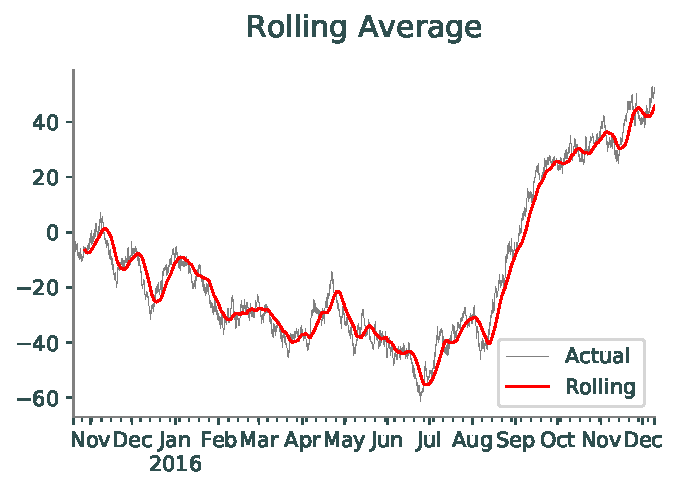
\includegraphics[width=\textwidth]{figures/moving_rolling.pdf}
    \caption{}
    \label{fig:pandas-ts-moving-rolling}
\end{subfigure}
%
\begin{subfigure}{.49\textwidth}
    \centering
    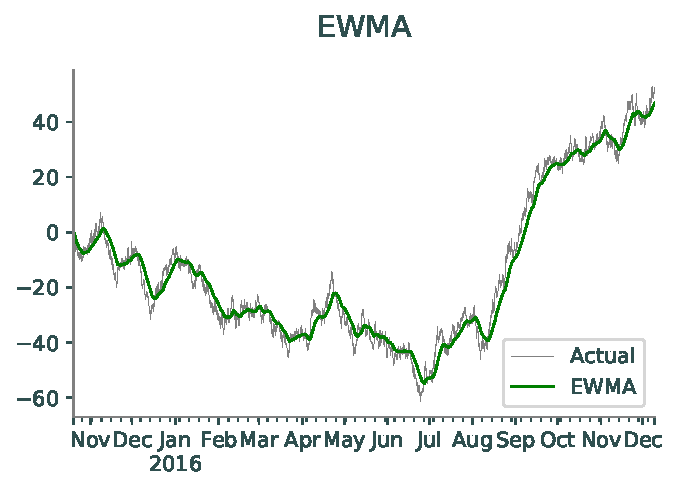
\includegraphics[width=\textwidth]{figures/moving_ewma.pdf}
    \caption{}
    \label{fig:pandas-ts-moving-ewma}
\end{subfigure}
\caption{Rolling average and EWMA.}
\end{figure}

\begin{lstlisting}
ax2 = plt.subplot(122)
s.plot(color="gray", lw=0.3, ax=ax2)
s.ewm(span=200).mean().plot(color='g', lw=1, ax=ax2)
ax2.legend(["Actual", "EWMA"], loc="lower right")
ax2.set_title("EWMA")
\end{lstlisting}
